\documentclass[aspectratio=169,11pt]{beamer}
\usetheme{Madrid}
\usepackage{graphicx}
\usepackage{booktabs}
\usepackage{tikz}
\usetikzlibrary{arrows.meta, positioning}
\definecolor{DeepPurple}{HTML}{211530}
\definecolor{RoyalPurple}{HTML}{6D28D9}
\definecolor{SoftPurple}{HTML}{F0EBFF}
\definecolor{MidPurple}{HTML}{9B70ED}
\setbeamercolor{structure}{fg=RoyalPurple}
\setbeamercolor{palette primary}{bg=DeepPurple,fg=white}
\setbeamercolor{palette secondary}{bg=RoyalPurple,fg=white}
\setbeamercolor{palette tertiary}{bg=DeepPurple,fg=white}
\setbeamercolor{frametitle}{bg=DeepPurple,fg=white}
\setbeamercolor{block title}{bg=RoyalPurple,fg=white}
\setbeamercolor{block body}{bg=SoftPurple,fg=DeepPurple}
\setbeamertemplate{navigation symbols}{}
\title[County Insights]{County Insights}
\subtitle{Reconstructing demographic profiles and exploring county planning choices}
\author[Olive Mideva Muloma]{Olive Mideva Muloma\\Admission number: 135792}
\date{\today}

\newcommand{\deploymentlink}{%
  \href{https://aml-capstone-ui.onrender.com/}{%
    \textcolor{RoyalPurple}{\nolinkurl{https://aml-capstone-ui.onrender.com/}}}}

\begin{document}
\begin{frame}
  \titlepage
  \vspace{-0.5em}
  \centering\small Experimental decision support using Kenya county population data
  \par\vspace{0.6em}
  \textbf{GitHub repository:}\\
  \href{https://github.com/olivemideva/capstone_project_aml.git}{%
    \textcolor{RoyalPurple}{\nolinkurl{github.com/olivemideva/capstone_project_aml.git}}}
  \par\vspace{0.3em}
  \textbf{Deployed application:}\\
  \deploymentlink
\end{frame}

\begin{frame}{The problem}
  \begin{block}{Planning with incomplete information}
    Missing population numbers can make it harder to compare counties and explore
    where services might be needed.
  \end{block}
  \begin{itemize}
    \item Can missing age--sex population cells be estimated from the available profile?
    \item How might different priorities change which counties are selected?
    \item Outputs are exploratory estimates, not official counts or funding decisions.
  \end{itemize}
\end{frame}

\begin{frame}{Data and preparation}
  \begin{columns}[T]
    \column{0.56\textwidth}
    \begin{itemize}
      \item Kenya's 47 county profiles, from a 2019 HDX HAPI age--sex extract.
      \item 42 age--sex cells per county: female and male, in five-year age bands and 100+.
      \item Source totals were checked, not assumed to be correct.
      \item 137 of 1,175 completed consistency checks were inconsistent.
    \end{itemize}
    \column{0.42\textwidth}
    \begin{block}{Avoiding leakage}
      Source aggregate totals and county identifiers are not demographic model predictors.
    \end{block}
    \small Source: project cleaning and consistency report.
  \end{columns}
\end{frame}

\begin{frame}{Experiment design}
  \begin{itemize}
    \item Split by county: \textbf{33 training, 7 validation, 7 reserved test} counties.
    \item Hide known values to simulate missing data: scattered cells, age blocks and
    whole-county blocks, at 10\%, 20\% and 40\%.
    \item Tune with county-grouped cross-validation; measure error only on hidden cells.
    \item Compare Random Forest, XGBoost and a masked autoencoder; also examine a
    training-county median reference.
  \end{itemize}
  \begin{alertblock}{Important}
    The final test split was not evaluated in the selected artifact; results below are
    validation results, not final test performance.
  \end{alertblock}
\end{frame}

\begin{frame}{Why these techniques?}
  \begin{block}{Reconstruction}
    Tree models can capture nonlinear relationships between age groups. The masked
    autoencoder learns a profile representation and tests whether aggregate constraints help.
  \end{block}
  \begin{block}{Planning}
    A weighted baseline offers an interpretable priority-based choice. NSGA-III explores
    alternative trade-offs across multiple objectives.
  \end{block}
  \small The autoencoder uses reported totals as extra training supervision; tree models do not.
  Comparisons therefore reflect different training information.
\end{frame}

\begin{frame}{Validation: model selection}
  \small Unweighted mean MAE across nine masking scenarios; lower is better.
  \vspace{0.7em}
  \begin{center}
  \begin{tabular}{lrr}
    \toprule
    Model family & Mean validation MAE & Selection \\
    \midrule
    Random Forest & 5,582 & Selected \\
    Masked autoencoder & 5,637 & \\
    XGBoost & 5,780 & \\
    \bottomrule
  \end{tabular}
  \end{center}
  \begin{itemize}
    \item MAE is the average absolute error in people per masked cell.
    \item Selection is based on seven validation counties, not all Kenyan counties.
    \item A small average difference does not establish a reliable winner.
  \end{itemize}
  \tiny Source: \texttt{models/selected/selection.json}; rounded to whole people.
\end{frame}

\begin{frame}{Results vary by missing-data scenario}
  \small Selected Random Forest on the validation split:
  \vspace{0.4em}
  \begin{center}
  \begin{tabular}{lrrrr}
    \toprule
    Scenario & Hidden cells & MAE & RMSE & $R^2$ \\
    \midrule
    Scattered, 10\% & 29 & 2,953 & 4,903 & 0.943 \\
    Scattered, 20\% & 59 & 4,509 & 7,157 & 0.924 \\
    Entire county, 40\% & 126 & 6,960 & 12,217 & 0.698 \\
    \bottomrule
  \end{tabular}
  \end{center}
  \begin{itemize}
    \item RMSE penalises large errors more strongly; $R^2$ compares with the evaluation mean.
    \item Error varies substantially by scenario; the median reference beat the selected
    model in three of nine validation scenarios.
  \end{itemize}
  \tiny Source: \texttt{reports/baselines/baseline\_validation.csv} and notebook diagnostics.
\end{frame}

\begin{frame}{Understanding the metrics}
  \begin{itemize}
    \item \textbf{MAE}: average absolute difference between estimated and known
    hidden values. A value of 2,953 means an average error of about 2,953 people
    per hidden age--sex cell, not per county.
    \item \textbf{RMSE}: square root of the average squared error; larger mistakes
    have more influence. It uses the same units as MAE.
    \item \textbf{$R^2$}: compares squared errors with predicting the evaluation
    cells' mean; 1 is perfect, 0 matches that reference, and negative is worse.
    It is not a percentage of correct predictions.
  \end{itemize}
  \small The 29 hidden cells in the first example come from seven validation
  counties; they are not 29 independent counties.
\end{frame}

\begin{frame}{Why the numbers are traceable}
  \begin{itemize}
    \item Fixed seed and county split; matching input hash and mask fingerprints
    check that model families were compared on the same hidden targets.
    \item The saved selected artifacts reproduce all nine validation MAEs; their
    unweighted average is 5,582.32 people per cell.
    \item The metrics implementation is checked against small known examples.
    A training-county median reference wins in three of nine scenarios.
    \item County-grouped cross-validation is used for tuning; the seven-county
    validation results shown here are a separate model-selection evaluation.
  \end{itemize}
  \begin{alertblock}{Reproducible does not mean universally accurate}
    Only seven validation counties, simulated gaps and an untouched test set:
    these checks cannot establish future performance or rule out overfitting.
  \end{alertblock}
\end{frame}

\begin{frame}{What influenced a prediction?}
  \begin{columns}
    \column{0.60\textwidth}
    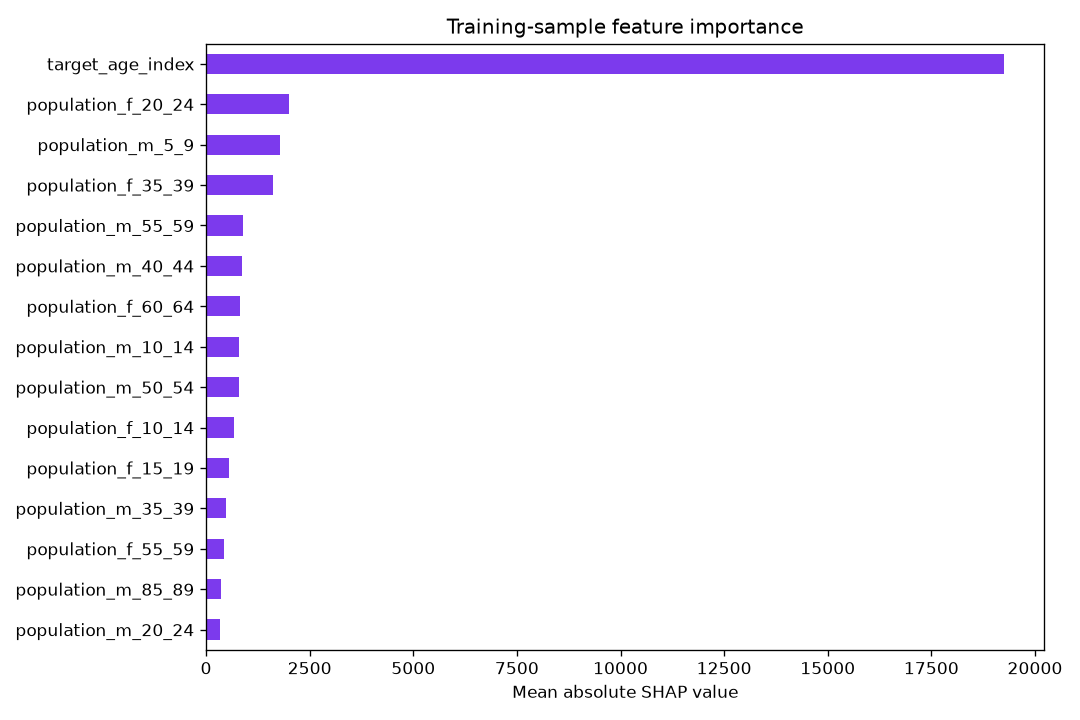
\includegraphics[width=\linewidth,height=0.68\textheight,keepaspectratio]{random_20_random_forest_shap.png}
    \column{0.38\textwidth}
    \small
    \begin{itemize}
      \item This training-sample SHAP plot is for scattered gaps at 20\%.
      \item The age group being estimated had the largest average contribution.
      \item Importance is not proof of causation or validation on new counties.
    \end{itemize}
  \end{columns}
\end{frame}

\begin{frame}{Exploring planning trade-offs}
  \begin{itemize}
    \item Uses \textbf{observed} profiles, not the reconstructed output.
    \item Example: select at most ten counties, treating each as one simulated cost unit.
    \item Compare shares of children, older people and the sum of county age-based
    dependency ratios.
    \item The third measure is an illustrative proxy, not a validated measure of fairness.
  \end{itemize}
  \begin{block}{One run, not a guarantee}
    The weighted grid produced 28 front solutions and NSGA-III produced 21.
    Their hypervolumes were 0.0421 and 0.0406 respectively for the stated reference point.
  \end{block}
  \tiny Source: \texttt{reports/prioritisation/summary.json}; seed 42, 200 generations.
\end{frame}

\begin{frame}{From data to an interactive service}
  \centering
  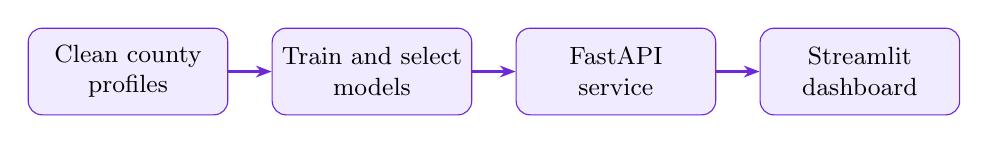
\begin{tikzpicture}[node distance=0.55cm, every node/.style={font=\small},
    box/.style={draw=RoyalPurple, fill=SoftPurple, rounded corners=5pt, minimum height=1.1cm, text width=2.3cm, align=center},
    arrow/.style={-{Stealth[length=2mm]}, thick, draw=RoyalPurple}]
    \node[box] (data) {Clean county\\profiles};
    \node[box,right=of data] (model) {Train and select\\models};
    \node[box,right=of model] (api) {FastAPI\\service};
    \node[box,right=of api] (ui) {Streamlit\\dashboard};
    \draw[arrow] (data) -- (model);
    \draw[arrow] (model) -- (api);
    \draw[arrow] (api) -- (ui);
  \end{tikzpicture}
  \vspace{1em}
  \begin{itemize}
    \item The dashboard supports exploring demographic estimates and planning choices.
    \item Docker Compose also starts Prometheus and Grafana for local monitoring.
    \item The Streamlit application and API are deployed on Render.
  \end{itemize}
\end{frame}

\begin{frame}{Limitations and responsible interpretation}
  \begin{itemize}
    \item Seven validation counties and simulated gaps limit generalisation; no final test score
    or absence of overfitting is established.
    \item Source inconsistencies and potential population changes can affect estimates.
    \item Whole-county gaps contain no observed demographic inputs; external evidence is needed.
    \item Costs are equal, simulated units; no actual budget, service coverage or causal impact
    is modelled.
    \item Predictions may be fractional; uploaded aggregate totals are not recalculated.
  \end{itemize}
\end{frame}

\begin{frame}{Next steps}
  \begin{enumerate}
    \item Freeze the methodology and evaluate once on the reserved test counties.
    \item Investigate source inconsistencies and evaluate on newer, independent data.
    \item Validate estimates and planning assumptions with domain stakeholders.
    \item Add real cost and need data before considering operational use.
  \end{enumerate}
  \vspace{1em}
  \textcolor{RoyalPurple}{\textbf{Takeaway:}} a reproducible prototype for exploring
  incomplete demographic data, not a substitute for official statistics or policy judgement.
\end{frame}

\begin{frame}{Evidence and reproducibility}
  \small
  \textbf{Project GitHub repository:}\\
  \href{https://github.com/olivemideva/capstone_project_aml.git}{%
    \textcolor{RoyalPurple}{\nolinkurl{https://github.com/olivemideva/capstone_project_aml.git}}}
  \par\vspace{0.3em}
  \textbf{Deployed application:}\\
  \deploymentlink
  \vspace{0.4em}
  \begin{itemize}
    \item Analysis and explanations: \texttt{notebooks/capstone\_analysis.ipynb}.
    \item Selection and artifacts: \texttt{models/selected/selection.json}.
    \item Validation metrics: \texttt{reports/baselines/baseline\_validation.csv}.
    \item Planning example: \texttt{reports/prioritisation/summary.json}.
    \item Source data: 2019 Kenya age--sex population extract, HDX HAPI.
    \item Pipeline, evaluation choices and local setup: project \texttt{README.md}.
  \end{itemize}
\end{frame}
\end{document}
